\section{Results}
The spectra were obtained

[Calibration] was then necessary,
in order [to derive the linear relationship] between [the channels] of the Multi Channel Analyser (MCA) thingy in which signal is detected 
and the corresponding energy values

This was accomplished using the known decay schems of the four sources.

\begin{figure}[h]
    \centering
    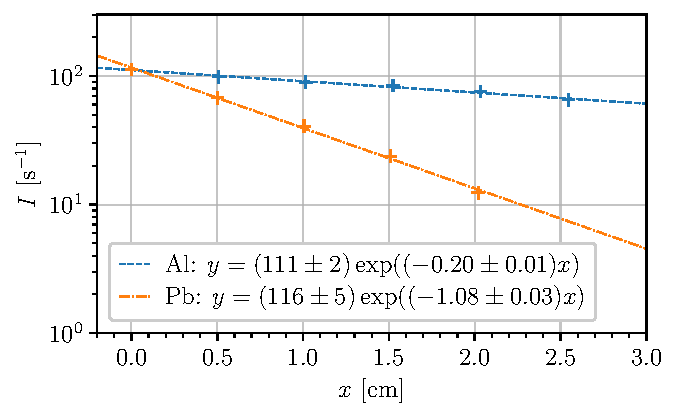
\includegraphics[scale=1]{figures/attenuation_coefficient.pdf}
    \caption{Attenuation coefficient}
    \label{fig:attenuation_coefficient}
\end{figure}